%%%%%%%%%%%%%%%%%%%%%%%%%%%%%%%%%%%%%%%%%%%%%%%%%%%
%% P3: Phenomenology of Particle Physics                         
%%
%% Author:  André Rubbia                   		 
%%
%% Figure 28.19 Predicted $y$-dependence of the differential cross-section of neutrino scattering.
%%
%% This work is licensed under the Creative Commons Attribution 4.0 International License. 
%% To view a copy of this license, visit http://creativecommons.org/licenses/by/4.0/ or 
%% send a letter to Creative Commons, PO Box 1866, Mountain View, CA 94042, USA.
%%
%%%%%%%%%%%%%%%%%%%%%%%%%%%%%%%%%%%%%%%%%%%%%%%%%%%

\documentclass[a4paper,10pt]{article}

\usepackage[T1]{fontenc}
\usepackage[utf8]{inputenc}
\usepackage{lmodern}
\usepackage[labelfont=bf]{caption}
\usepackage{upgreek}

\usepackage{amssymb}
\usepackage{amsmath}
\usepackage{mathtools}

\usepackage{tikz}
\usepackage{pgfplots}
\pgfplotsset{compat=1.17}
\usepgfplotslibrary{ternary}
\usepgfplotslibrary{fillbetween}
\usepgfplotslibrary{external}

\def\d{\mathrm{d}}
\setlength{\oddsidemargin}{-1.0cm}
\setlength{\evensidemargin}{-1.0cm}
\setlength{\textheight}{25cm}
\setlength{\textwidth}{18cm}

\pgfkeys{/pgf/number format/.cd,1000 sep={}}

\begin{document}

%%%%%%%%%%%%%%%%   FIGURE  %%%%%%%%%%%%%%%%%%%%%%%%%%%%%%
\begin{figure}[htb]
	\centering
\begin{tikzpicture}[scale=1.]
\begin{axis}[xmin=0, xmax=1,
	xtick={0,0.5,1},
	ymin=0, ymax=0.55,
	title=$\nu {\cal N}\rightarrow \ell^- + X$,
	xlabel=$y$,
	ylabel=$\d\sigma/\d y$ in units of $G_F^2 s/2\pi$,
]
	\addplot[domain=0:1,blue,very thick] {0.41+0.08*(1-x)^2};
	\addplot[domain=0:1,blue,dashed,very thick] {0.41};
	\node[red] at (axis cs:0.5,0.2) {\Large $u+d$};
	\node[red] at (axis cs:0.5,0.5) {\Large $\bar u+\bar d$};
	\draw[red,<-, very thick] (axis cs:0.2,0.44) -- (axis cs:0.4,0.475);
\end{axis}
\end{tikzpicture}
\caption{Predicted $y$-dependence of the differential cross-section
of neutrino scattering.}
\end{figure}
%
%%%%%%%%%%%%%%%%   END FIGURE  %%%%%%%%%%%%%%%%%%%%%%%%%%%%%%
%


\end{document}
